\chapter{Zielsetzung}

\begin{itemize}
	\item Erstellung eines Simulators zur 3D-Visualisierung von Achterbahnen
		\begin{itemize}
			\item Physikalisch korrekte Wiedergabe
			\item Bodengrundfläche, 2 parallele Schienen, Querträger 
		\end{itemize}
	\item 2D-Visualisierung für Beschleunigungsdaten
	\item[$\Rightarrow$] Ingenineursmäßige Konstruktion einer Achterbahn
\end{itemize}

\begin{figure}[!h]
	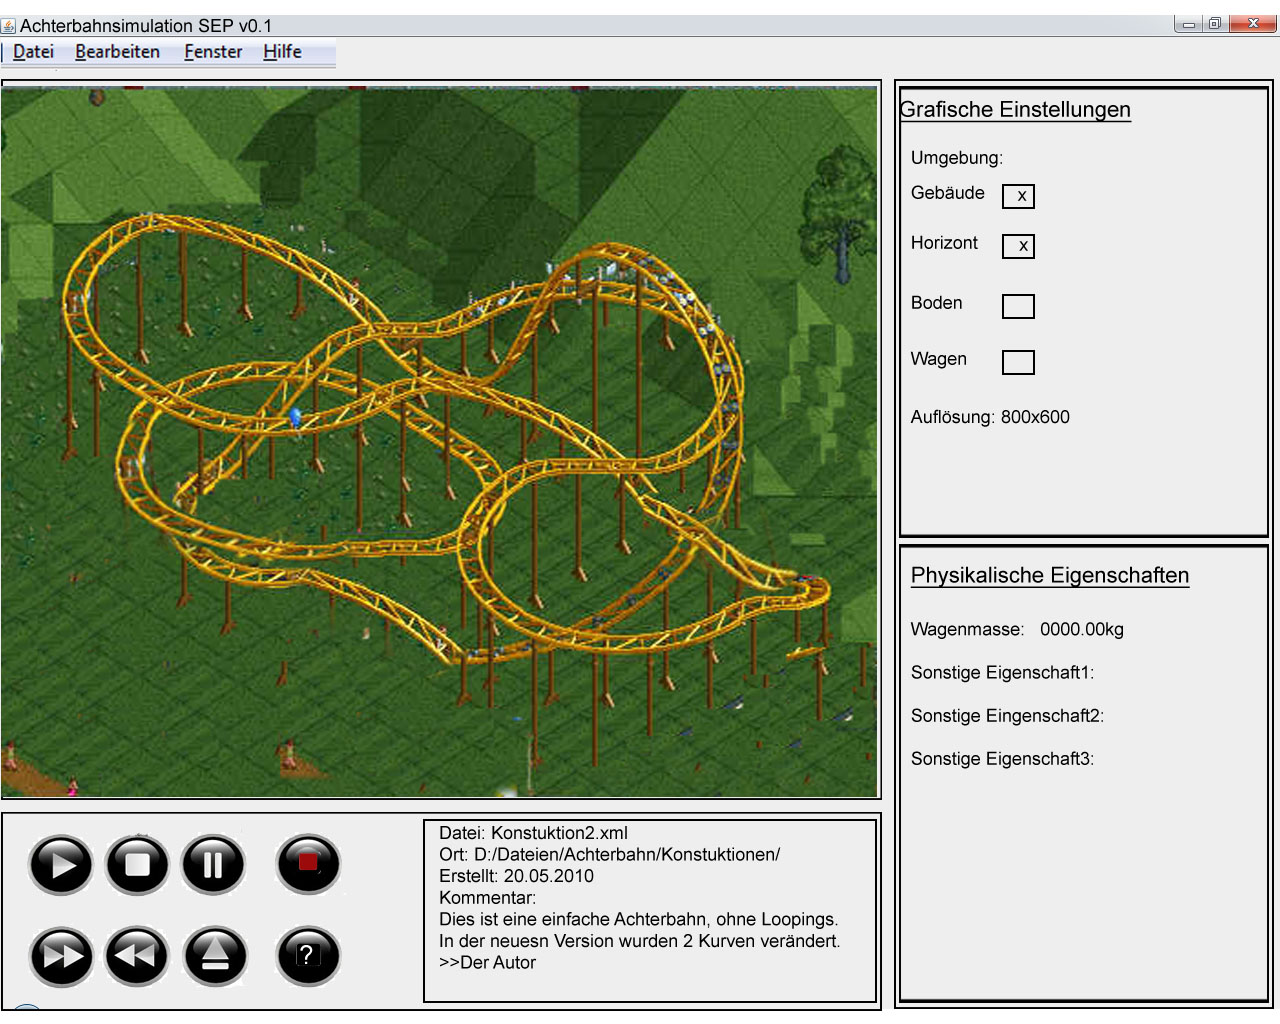
\includegraphics[width=\linewidth]{bilder/GUI_v3}
	\caption{Vor dem Starten}
\end{figure}
\begin{figure}[!h]
	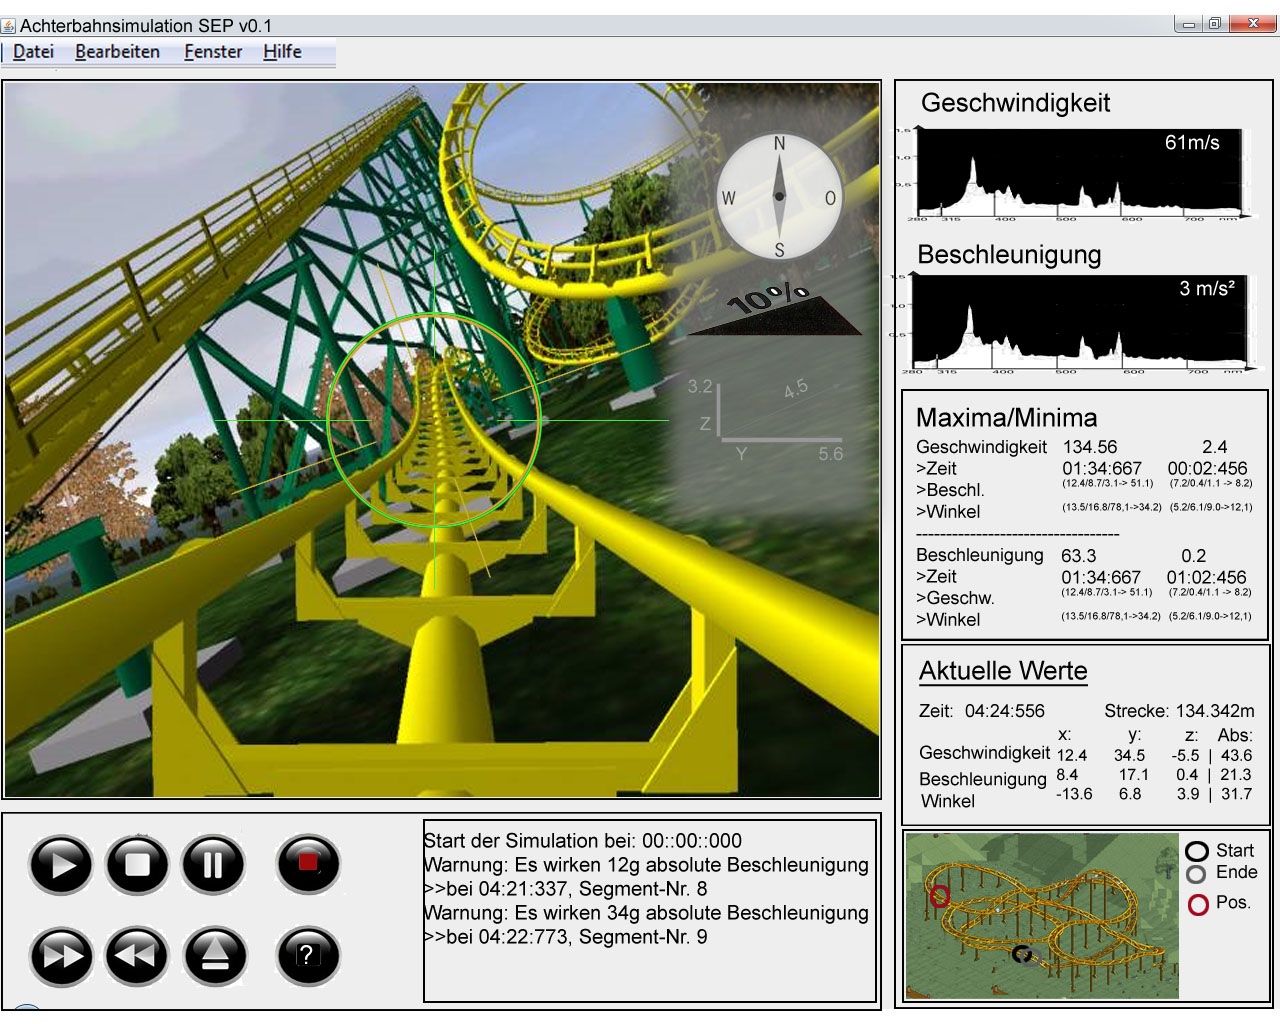
\includegraphics[width=\linewidth]{bilder/GUI_v2}
	\caption{Während der Simulation}
\end{figure}